

\section{Objetivo}
Comprender el algoritmo de búsqueda con retractación (\textit{backtrack}) y su relación con recursión. Llevar a cabo su implementación en la construcción de laberintos. Entender la forma de representar la lógica de la construcción del laberinto y su visualización. \par

\section{Introducci\'on}
\textbf{Retractación} es un algoritmo para encontrar soluciones en problemas computacionales donde se encuentran varios candidatos parciales de solución que se van descartando conforme avanza el algoritmo o la búsqueda.

El problema más clásico de la aplicación de retractación es el problema de las \textbf{ocho reinas} que consiste en colocar ocho reinas en un tablero de ajedrez convencional de manera que ninguna ataque a las demás. En cada paso del algoritmo se agrega una reina a una casilla y se verifica que no ataque a las \textbf{k} reinas del tablero. Cuando no se cumple esta condición, se vuelve a una solución válida previa y se continúa probando hasta que satisfaga que no se ataquen ninguna de las reinas del tablero.\par

La aplicación de la técnica de retractación sólo tiene sentido en problemas que involucran soluciones parciales. Hay que notar que es una manera más eficiente que el uso de fuerza bruta, ya que se descartan muchas posibilidades de que no cumplen los requisitos de ser solución del problema.

Conceptualmente, retractación es similar a la búsqueda en profundidad en árboles. Considerando que cada nodo en el árbol de búsqueda es una posible solución parcial del problema, la forma de recorrerlo es mediante recursión; podando o descartando subárboles que no son válidos como solución.\par


\section{Desarrollo e implementaci\'on}

\noindent Se desarrollará una aplicación que genera laberintos, usando una interfaz gráfica.

\subsection{Algoritmo de construcci\'on del laberinto}


En laboratorio se realizó la definición y discusión del problema.
Como recurso se empleó el ejemplo de la siguiente página para ver la construcción (primer ejemplo: ``\textit{recursive backtracker}''):
\href{http://weblog.jamisbuck.org/2011/2/7/maze-generation-algorithm-recap}{Recursive Backtracker}
\footnote{http://weblog.jamisbuck.org/2011/2/7/maze-generation-algorithm-recap}
También hay una liga sobre el algoritmo y una implementación hecha en lenguaje Ruby:
\href{http://weblog.jamisbuck.org/2010/12/27/maze-generation-recursive-backtracking}{Maze generation}
\footnote{http://weblog.jamisbuck.org/2010/12/27/maze-generation-recursive-backtracking}

\noindent A continuación se explica la construcción del laberinto:

\begin{enumerate}
  \item El algoritmo comienza con un tablero de celdas de tamaño N x M.
    \begin{figure}[h!]
      \centering
      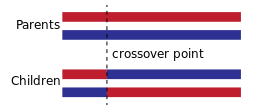
\includegraphics[width=0.2\textwidth]{retractacion/screen1.png}
      \caption{Ejemplo con N=6 y M=6.}
      \label{fig:tablero1}
    \end{figure}
  \item Se elige una celda aleatoriamente como la celda actual, se marca como visitada y se agrega al stack.
    \begin{figure}[h!]
      \centering
      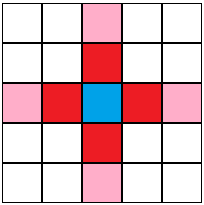
\includegraphics[width=0.2\textwidth]{retractacion/screen2.png}
      \caption{}
      \label{fig:tablero2}
    \end{figure}
  \item Se elige de manera aleatoria una dirección hacia donde moverse, esto consiste en elegir una casilla adyacente que no haya sido visitada. Dependiendo de la dirección elegida se debe borrar la pared correspondiente. Se marca como visitada la celda y se actualiza la celda actual.
    \pagebreak
    \begin{figure}[h!]
      \centering
      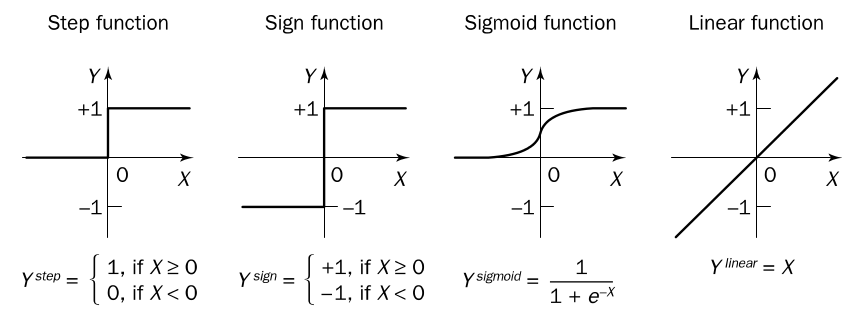
\includegraphics[width=0.2\textwidth]{retractacion/screen3.png}
      \caption{Ejemplo donde se elige la celda de la derecha. Se borra la pared entre las celdas y se marca la nueva celda actual (color rojo).}
      \label{fig:tablero3}
    \end{figure}
  \item El paso anterior se repite hasta que ya no haya direcciones por elegir, es decir, se queda encerrada la celda actual.
    \begin{figure}[h!]
      \centering
      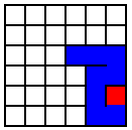
\includegraphics[width=0.2\textwidth]{retractacion/screen4.png}
      \caption{Tras algunos movimientos, la celda actual ya no puede seguir moviéndose.}
      \label{fig:tablero4}
    \end{figure}
  \item Estando encerrados sin poder elegir una celda adyacente sin visitar, se procede a hacer un pop al stack de celdas para cambiar la posición de la celda actual y repetir el algoritmo desde el paso 3 hasta recorrer todo el tablero de celdas.
    \begin{figure}[h!]
      \centering
      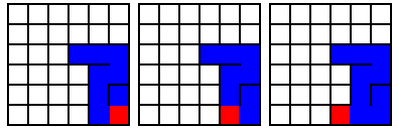
\includegraphics[width=0.6\textwidth]{retractacion/screen5.png}
      \caption{Ejemplo de un retroceso usando el stack y cambiando la celda actual.}
      \label{fig:tablero5}
    \end{figure}
    \pagebreak
    \begin{figure}[h!]
      \centering
      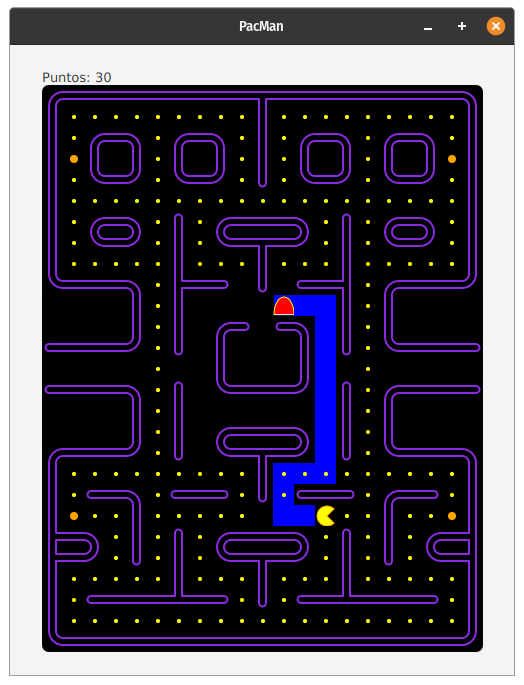
\includegraphics[width=0.6\textwidth]{retractacion/screen6.png}
      \caption{Ejemplo tras varios pasos del algoritmo hasta cubrir todo el tablero.}
      \label{fig:tablero6}
    \end{figure}
\end{enumerate}


\subsection{Implementaci\'on}

Se debe implementar tanto la lógica de construcción del laberinto como su visualización. Se recomienda usar \classname{Processing} ya que solo requiere usar las primitivas de dibujo: \classname{stroke()}, \classname{line()}. Adicionalmente también pueden usar: \classname{fill()}, \classname{rect()}. Recomendable usar los siguientes métodos para una adecuada visualización: \classname{background()}, \classname{size()}.



\section{Requisitos y resultados}

Para llevar a cabo la evaluación de esta práctica es necesario implementar la construcción del laberinto usando retractación. Empleen como estructura auxiliar durante la construcción una pila o stack.

La implementación debe ser lo más generalizada y robusta posible, es decir, se deben definir parámetros o valores para determinar el ancho y largo del laberinto.

No olviden documentar su código. De preferencia utilicen el estándar de \classname{JavaDoc}, de no hacerlo, al menos describan de manera breve, clara y concisa el funcionamiento de sus métodos. Si omiten documentación en su código les afectará negativamente en su calificación.

El ejemplo visto en laboratorio se construye en tiempo de ejecución. Es deseable que se muestre esta construcción pero no es necesaria. Es válido mostrar el resultado final aunque no se visualice la construcción.

Si todo se implementa correctamente debe ser posible generar diferentes tamaños de laberintos.



% \subsection{Agradecimientos}
% \noindent Esta práctica fue realizada originalmente por Rodrigo Eduardo Colín Rivera (animeroy@gmail.com). Se hicieron algunas modificaciones, pero sigue mereciendo crédito por su labor. \\\\

